\clearpage
\subsubsection{job}
\begin{table}[H]
  \centering
  \begin{tabular}{|c|l|l|} \hline
    モジュール名                & \multicolumn{2}{l|}{job.dart}                                                                         \\ \hline
    モジュール概要               & \multicolumn{2}{p{12cm}|}{求人画面を表示するモジュール}                                                             \\ \hline
    責任者                   & \multicolumn{2}{l|}{新谷光城}                                                                             \\ \hline
    \multirow{7}{*}{構成要素} & クラス名                                                 & JobRouterPage                                  \\ \cline{2-3}
                          & クラス種類                                                & extends AppRouter                              \\ \cline{2-3}
                          & 処理概要                                                 & \multicolumn{1}{p{12cm}|}{JobをアクセスするためのRouter} \\ \cline{2-3}
                          & 入力                                                   & なし                                             \\ \cline{2-3}
                          & 出力                                                   & Route                                          \\ \cline{2-3}
                          & \multicolumn{2}{l|}{他クラス・関数との関係}                                                                      \\ \cline{2-3}
                          & \multicolumn{2}{p{14cm}|}{なし}                                                                         \\ \hline
    \multirow{7}{*}{構成要素} & クラス名                                                 & Job                                            \\ \cline{2-3}
                          & クラス種類                                                & extends StatelessWidget                        \\ \cline{2-3}
                          & 処理概要                                                 & \multicolumn{1}{p{12cm}|}{求人画面を動的にするクラス}       \\ \cline{2-3}
                          & 入力                                                   & なし                                             \\ \cline{2-3}
                          & 出力                                                   & Widget                                         \\ \cline{2-3}
                          & \multicolumn{2}{l|}{他クラス・関数との関係}                                                                      \\ \cline{2-3}
                          & \multicolumn{2}{p{14cm}|}{job.dartのJobStateクラスを組み込む}                                                  \\ \hline
    \multirow{7}{*}{構成要素} & クラス名                                                 & JobState                                       \\ \cline{2-3}
                          & クラス種類                                                & extends StatelessWidget                        \\ \cline{2-3}
                          & 処理概要                                                 & \multicolumn{1}{p{12cm}|}{求人画面の状態を返すクラス}       \\ \cline{2-3}
                          & 入力                                                   & なし                                             \\ \cline{2-3}
                          & 出力                                                   & State                                          \\ \cline{2-3}
                          & \multicolumn{2}{l|}{他クラス・関数との関係}                                                                      \\ \cline{2-3}
                          & \multicolumn{2}{p{14cm}|}{
      post\_list.dartのPostListクラスを組み込む
      \newline else\_list.dartのElseListクラスを呼び出すことでお気に入りイベント一覧画面、閲覧履歴画面を表示
      \newline search\_post.dartのSearchPostを呼び出すことで検索結果画面を表示
    \newline job\_post\_write.dartのJobPostWriteクラスを呼び出すことで求人詳細画面を表示}                                                              \\ \hline
  \end{tabular}
\end{table}

\begin{figure}[H]
  \centering
  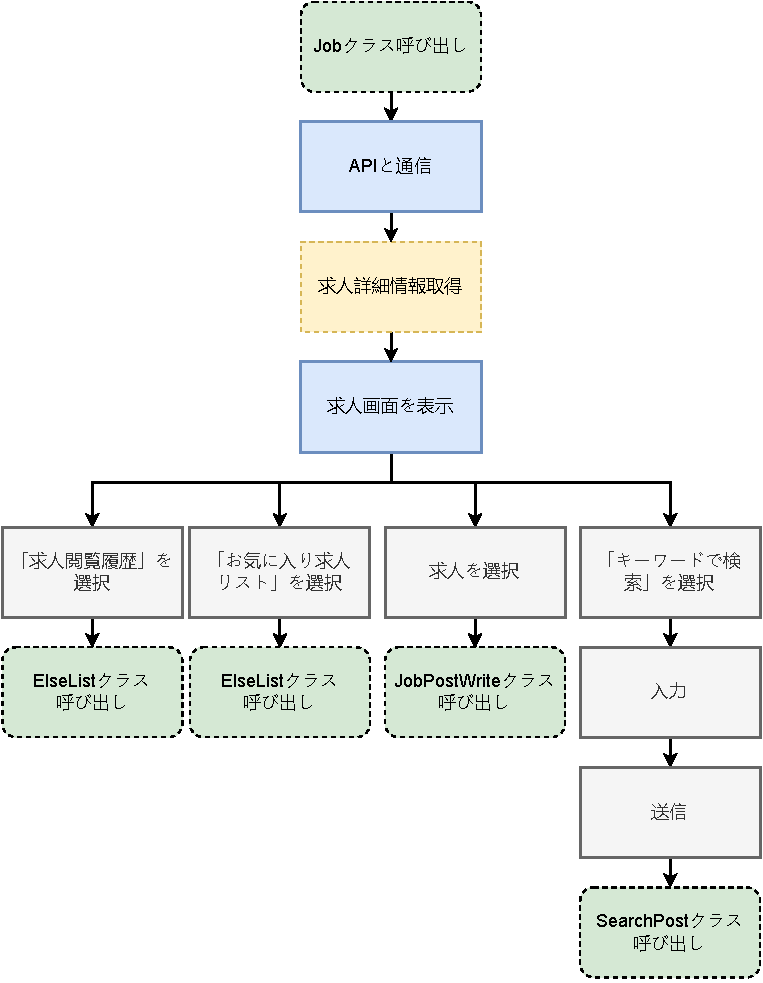
\includegraphics[width=16cm]{./images/internal-design/state_change_diagram/job/job.pdf}
  \caption{job.dartの状態遷移図}
\end{figure}


\begin{table}[H]
  \centering
  \begin{tabular}{|c|l|l|} \hline
    モジュール名                & \multicolumn{2}{l|}{job\_post\_write.dart}                                                        \\ \hline
    モジュール概要               & \multicolumn{2}{p{12cm}|}{イベント広告内容記述画面を表示するモジュール}                                                 \\ \hline
    責任者                   & \multicolumn{2}{l|}{新谷光城}                                                                         \\ \hline
    \multirow{7}{*}{構成要素} & クラス名                                              & JobPostWrite                                  \\ \cline{2-3}
                          & クラス種類                                             & extends StatelessWidget                       \\ \cline{2-3}
                          & 処理概要                                              & \multicolumn{1}{p{12cm}|}{求人広告内容記述画面を表示するクラス} \\ \cline{2-3}
                          & 入力                                                & なし                                            \\ \cline{2-3}
                          & 出力                                                & Widget                                        \\ \cline{2-3}
                          & \multicolumn{2}{l|}{他クラス・関数との関係}                                                                  \\ \cline{2-3}
                          & \multicolumn{2}{p{14cm}|}{
      change\_general\_corporation.dartのChangeGeneralCorporationプロバイダを組み込む
      \newline job\_fee\_select.dartのJobPostInfoプロバイダを組み込む
      \newline title\_appbar.dartのTitleAppBarクラスを組み込む
      \newline post\_conf.dartのPostConfクラスを呼び出し投稿確認オーバーレイを表示
      \newline return\_write.dartのReturnWriteクラスを呼び出し必須内容記入漏れ注意オーバーレイを表示
      \newline move\_conf.dartのMoveConfクラスを呼び出し投稿中に移動確認オーバーレイを表示
    \newline 戻るボタンの選択で前のモジュールに戻る}                                                                                             \\ \hline
  \end{tabular}
\end{table}

\begin{figure}[H]
  \centering
  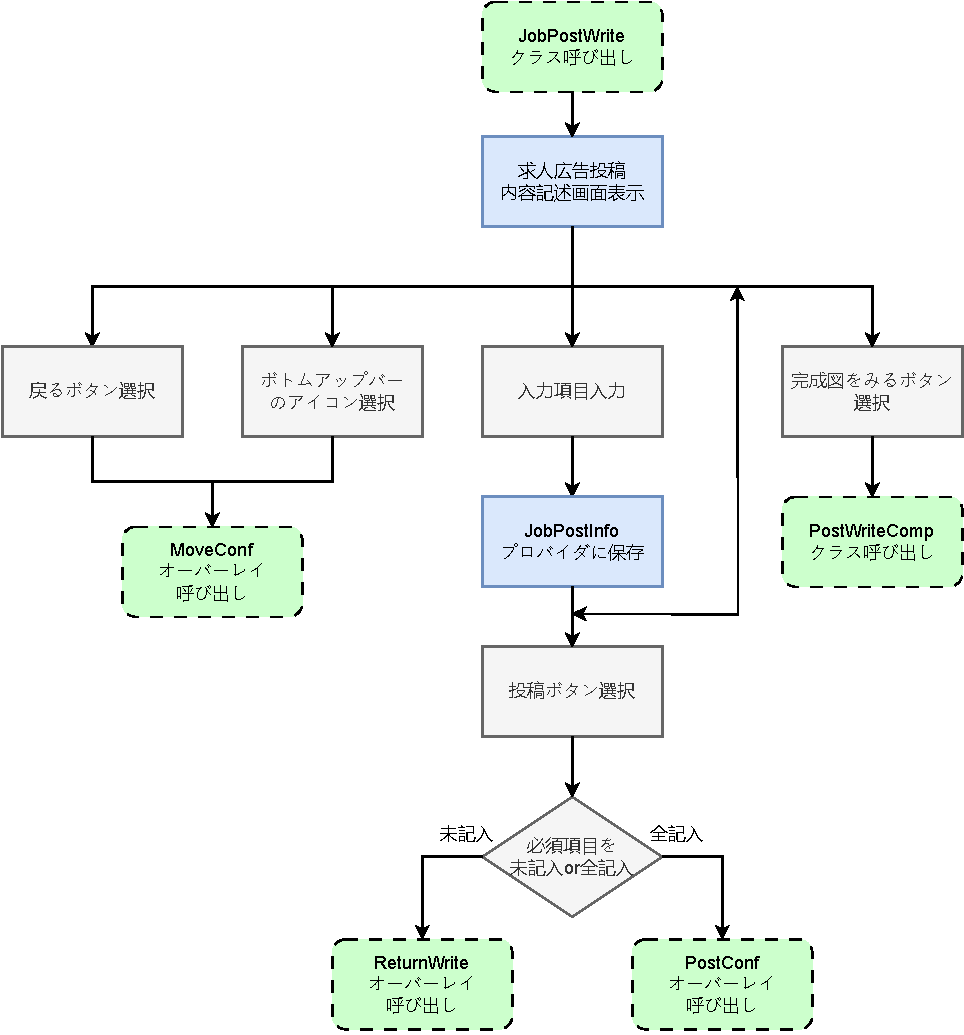
\includegraphics[width=17cm]{./images/internal-design/state_change_diagram/job/job_post_write.pdf}
  \caption{job\_post\_write.dartの状態遷移図}
\end{figure}




\begin{table}[H]
  \centering
  \begin{tabular}{|c|l|l|} \hline
    モジュール名                & \multicolumn{2}{l|}{job\_post\_detail.dart}                                                                              \\ \hline
    モジュール概要               & \multicolumn{2}{p{12cm}|}{求人広告詳細画面を表示するモジュール}                                                                            \\ \hline
    責任者                   & \multicolumn{2}{l|}{新谷光城}                                                                                                \\ \hline
    \multirow{7}{*}{構成要素} & クラス名                                                                    & JobPostDetail                                  \\ \cline{2-3}
                          & クラス種類                                                                   & extends StatelessWidget                        \\ \cline{2-3}
                          & 処理概要                                                                    & \multicolumn{1}{p{12cm}|}{求人広告詳細画面を動的に変更するクラス} \\ \cline{2-3}
                          & 入力                                                                      & Map$<$String, dynamic$>$ info                  \\ \cline{2-3}
                          & 出力                                                                      & Widget                                         \\ \cline{2-3}
                          & \multicolumn{2}{l|}{他クラス・関数との関係}                                                                                         \\ \cline{2-3}
                          & \multicolumn{2}{p{14cm}|}{job\_post\_detail.dartのJobPostDetailクラスを組み込む}                                                  \\ \hline
    \multirow{7}{*}{構成要素} & クラス名                                                                    & JobPostDetailState                             \\ \cline{2-3}
                          & クラス種類                                                                   & extends StatelessWidget                        \\ \cline{2-3}
                          & 処理概要                                                                    & \multicolumn{1}{p{12cm}|}{求人広告詳細画面の状態を返すクラス}   \\ \cline{2-3}
                          & 入力                                                                      & なし                                             \\ \cline{2-3}
                          & 出力                                                                      & State                                          \\ \cline{2-3}
                          & \multicolumn{2}{l|}{他クラス・関数との関係}                                                                                         \\ \cline{2-3}
                          & \multicolumn{2}{p{14cm}|}{
      change\_general\_corporation.dartのChangeGeneralCorporationプロバイダを組み込む
      \newline title\_appbar.dartのTitleAppBarクラスを組み込む
      \newline impression.dartのImpressionクラスを呼び出しインプレッション画面を表示
      \newline post\_mem\_list.dartのPostMemListクラスを呼び出し応募者一覧画面を表示
      \newline event\_post\_write.dartのEventPostWriteクラスを呼び出しイベント広告内容変更画面を表示
    \newline delete\_conf.dartのDeleteConfクラスを呼び出し投稿削除確認オーバーレイを表示}                                                                                    \\ \hline
  \end{tabular}
\end{table}

\begin{figure}[H]
  \centering
  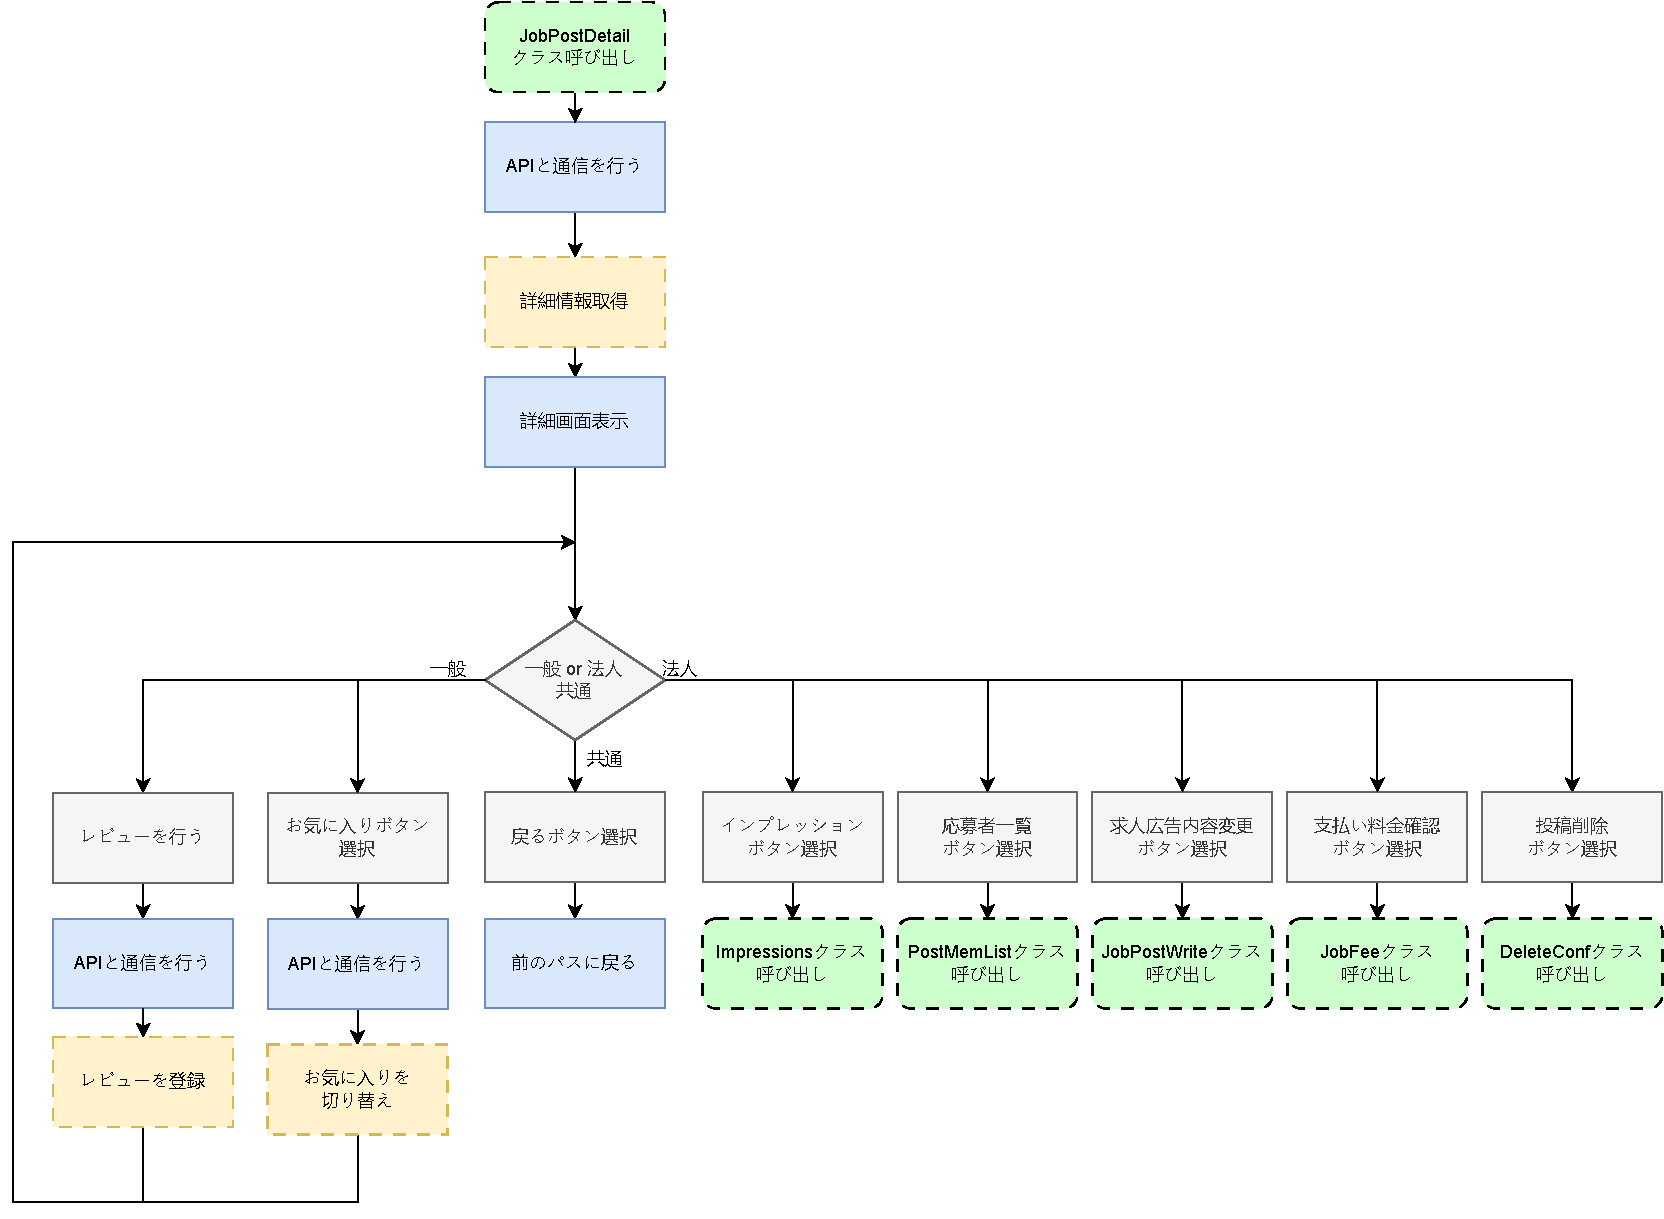
\includegraphics[width=18cm]{./images/internal-design/state_change_diagram/job/job_post_detail.pdf}
  \caption{job\_post\_detail.dartの状態遷移図}
\end{figure}